\documentclass[a4paper]{article}
\usepackage{t1enc}
\usepackage[magyar]{babel}
\usepackage{fullpage}
\usepackage{hyperref}
\usepackage{csquotes}
\usepackage{graphicx}

\selectlanguage{magyar}

\author{Uszkay Balázs}
\title{NHF specifikáció}

\hypersetup{colorlinks=true, linkcolor=blue}

\graphicspath{{./img/}}

\newcommand{\stacc}{{\it Stacc }}


\begin{document}
\maketitle
\section*{
\href{https://www.github.com/ubalu/stacc}{Stacc} (és a számítástudomány két legnehezebb problémája)
\footnote{Phil Karlton szerint két nehéz dolog van a számítástudományban: a gyorsítótár-érvénytelenítés és dolgok elnevezése.}
}

A \stacc egy kreatívan elnevezett, verem alapú konkatenatív, interpretált, általános célú programozási nyelv. Az inspirációt a \href{https://en.wikipedia.org/wiki/Forth_(programming_language)}{Forth} és a \href{https://https://factorcode.org/}{Factor} nyelvek adták.

\subsection*{Nyelvi elemek}
Egy \stacc program egymástól whitespace-szel elválasztott {\it szavakból} áll. Ezek jobbról balra kerülnek végrehajtásra. Szónak számít minden karaktercsoport, amelyek közt fehér tér van, kivétel a string konstans, amely \verb|"|-től (\verb|U+0022|) \verb|"|-ig tart. Ezek a szavak a központi vermen operálnak. Kommentek \verb|--|~-től a sor végéig tartanak.

A veremre helyezéshez (\verb|push|) nem tartozik külön szó, ez automatikusan megtörténik, amikor konstansba fut a program.

\subsection*{Adattípusok}
A program futás közben az adatokat a veremben tárolja. Ezek az adatok az alábbi típusúak lehetnek:
\begin{itemize}
\item {\bf integer:} 64-bites előjeles egész.\\
	{\bf Pl.:} \verb|-1 10 9223372036854775807|
\item {\bf float:} 64-bites lebegőpontos szám (\href{https://en.wikipedia.org/wiki/IEEE_754}{double}).\\
	{\bf Pl.:} \verb|27 -3.2 6.022e+23|
\item {\bf list:} Heterogén lista, más elemeket tartalmaz. \verb|{| szótól (\verb|U+007B|) \verb|}| szóig (\verb|U+007D|) tart.\\
	{\bf Pl.:} \verb|{ 1 2 3 4 } { { "alma" 213.3 } { } }|
\item {\bf string:} Karakterek listája, \verb|"|-től (\verb|U+0022|) \verb|"|-ig tart. A listák műveletei ugyanúgy érvényesek.\\
	{\bf Pl.:} \verb|"Tudja, hol szeret a cápa" "kecske" ""|
\item {\bf block:} Futtatható blokkok, egyfajta anonim függvények. Ezek segítségével lehet például if-else, ciklus stb. control flow-t megvalósítani. \verb|`[`| szótól (\verb|U+005B|) \verb|`]`| szóig (\verb|U+005D|) tart.\\
	{\bf Pl.:} \verb|0 < [ sqrt 2 * ] [ dup * ] if --| ez a program negatív számokon máshogy operál, mint pozitívakon
\item {\bf ident:} Olyan szó, amely valamilyen függvényre hivatkozik. Létrehozni a \verb|'| (\verb|U+0027|) karakterrel lehet, azaz a szó első karaktere \verb|'| kell, hogy legyen. \\
	{\bf Pl.:} \verb|[ 2 < [ drop 1 ] [ dup -1 + 'fac call * ] if ] 'fac :|\\
{\bf Megjegyzés. } A fenti kódrészletben szereplő \verb|:| szó névhez ({\bf 'ident}) köt egy blokkot ({\bf \{block\}}), azaz függvényt definiál. 
\end{itemize}
\pagebreak
\subsection*{Beépített primitívek}
\emph{Ez a szakasz nagyon megváltozhat a végleges beadásig!} \\

Az itt felsorolt primitív szavak egyből használhatók, ezeket definiálni nem kell. A \verb|( -- )| jelölés a Forth és a Factor által is használt (az előbbi által csak konvencióként) {\it veremjelölés} (stack notation), ahol a  \verb|--| bal és jobb oldala sorrendben a szó végrehajtása előtti és utáni verem állapotot jellemzi. Ilyenkor csak a legfelső $n$ elemet mutatjuk (hiszen csak ezek számítanak), a fent említett nyelvekhez képest annyi kiegészítéssel, hogy én a blokkokat és a neveket kiemelten jelölöm. Ezért például a \verb|:| szó veremjelölése: $$\verb|({block} 'ident -- )|,$$ hiszen ez a szó elnyeli a verem tetején lévő blokkot és nevet. A verem teteje jobbra van, így a \verb|rot| szó jelölése, $$\verb|(a b c -- b c a)|,$$ azt mutatja, hogy felülről harmadik elem kerül a stack tetejére.
\subsubsection*{I/O:}
\begin{itemize}
\item \begin{verbatim}. (a -- )\end{verbatim} Kiírja a stack legfelső elemét és ejti azt.
\item \begin{verbatim}S. (... -- ...)\end{verbatim} (Debug jellegű kiírás) kiírja a stack nagyságát és összes elemét.\\
Példa: \begin{verbatim}1 2 'nev [ dup * 2 + ] "árvíztűrő tükörfúrógép" { 1 2 "alma" 4 } S.
<5>
1
2
'nev
[<block>]
"árvíztűrő tükörfúrógép"
{<4-list>}
\end{verbatim}
\end{itemize}

\subsubsection*{Aritmetika, műveletek:}
\begin{itemize}
\item \begin{verbatim}+ (n1 n2 -- sum)
- (n1 n2 -- n1-n2)
* (n1 n2 -- prod)
/ (n1 n2 -- n1/n2)
% (n1 n2 -- n1%n2)
divmod (n1 n2 -- n1/n2 n1%n2)
pow (n1 n2 -- n1^n2)\end{verbatim} Bináris aritmetikai műveletek. \verb|%| a modulus operátor.
Stringeken a \verb|+| konkatenálásként működik.

\item \begin{verbatim}sqrt (n -- r)
sin (n -- r)
cos (n -- r)
tan (n -- r)
arcsin (n -- r)
arccos (n -- r)
arctan (n -- r)\end{verbatim} Unáris műveletek.

\item \begin{verbatim}inc (a -- a')
dec (a -- a')\end{verbatim} Eggyel növeli, ill. csökkenti a verem legfelső elemét.

\item \begin{verbatim}and (bool1 bool2 -- bool)
or (bool1 bool2 -- bool)
xor (bool1 bool2 -- bool)
not (bool -- bool)
\end{verbatim} Boole-algebrai műveletek. A \verb|false|-t a \verb|0| egész, a \verb|true|-t pedig a \verb|-1| (avagy nem \verb|0|) jelöli (emiatt jelenleg a \verb|not| egészekre a negálás).
\end{itemize}

\subsubsection*{Listaműveletek}
\begin{itemize}
\item \verb|len ({list} -- n)|\\ Visszaadja egy lista hosszát.
\item \verb|append ({list} item -- {list'})|\\ Végére illesztés
\item \verb|prepend ({list} item -- {list'})|\\ Elejére illesztés
\item \verb|insert ({list} index item -- {list'})|\\ Pozícióba illesztés.
\item \verb|each ({list} [block] -- ...)|\\ Művelet elemenként.
\item \verb|map ({list} [block] -- {list'})|\\ Művelet végrehajtása minden elemen.
\item \verb|filter ({list} [block] -- {list'})|\\ Elemek szűrése feltétel alapján.
\item \verb|reduce ({list} init [block] -- result)|\\ Redukció (\href{https://en.wikipedia.org/wiki/Fold_(higher-order_function)}{fold}).
\item \verb|reduce1 ({list} [block] -- result)|\\ Kezdőérték nélküli redukció.
\item \verb|scan ({list} init [block] -- {result})|\\ Folytonos redukció (\href{https://en.wikipedia.org/wiki/Prefix_sum#Scan_higher_order_function}{scan}).
\item \verb|scan1 ({list} [block] -- {result})|\\ Kezdőérték nélküli \verb|scan|.
\item \verb|first ({list} -- item)|\\ Első elem.
\item \verb|last ({list} -- item)|\\ Utolsó elem.
\item \verb|take ({list} n -- {list'})|\\ Első \verb|n| elem.
\item \verb|drop ({list} n -- {list'})|\\ Lista az első \verb|n| elem nélkül.
\item \verb|iota (n -- {list})|\\ Számok listája 1-től \verb|n|-ig.
\end{itemize}

\subsubsection*{Stringműveletek}
\begin{itemize}
\item \verb|upper ("str" -- "STR")|\\		Nagybetűssé tétel.
\item \verb|lower ("STR" -- "str")|\\		Kisbetűssé tétel.
\item \verb|find ("str" "sub" -- pos)|\\	Megkeresi \verb|"sub"| első pozícióját \verb|"str"|-ben.
\item \verb|count ("str" "sub" -- n)|\\		Visszaadja \verb|"sub"| darabszámát \verb|"str"|-ben.
\end{itemize}

\subsubsection*{Összehasonlítás: }
\begin{itemize}
\item \begin{verbatim}= (a b -- bool)
<  (a b -- bool)
<= (a b -- bool)
>  (a b -- bool)
>= (a b -- bool)
!= (a b -- bool)
\end{verbatim} Összehasonlítások. Irreflexív összehasonlításoknál a verem tetején levő kerül \textquote{jobbra}.\\ Példa: \begin{verbatim}2 3 < .
-1 -- 2 < 3, igaz
4 10 >= .
0 -- 4 >= 10, hamis\end{verbatim}
\end{itemize}

\subsubsection*{Verem kezelés: }
\begin{itemize}
\item \verb|<|{\it konstans}\verb|>| \verb|( -- a)|\\ Konstans felrakása a veremre.
\item \begin{verbatim}dup (a -- a a)\end{verbatim} {\it Duplicate}, a legfelső érték megduplázása.
\item \begin{verbatim}2dup (a b -- a b a b)\end{verbatim} {\it 2-Duplicate}, a felső elempár duplázása.
\item \begin{verbatim}swap (a b -- b a)\end{verbatim} A felső két érték cseréje.
\item \begin{verbatim}2swap (a b c d -- c d a b)\end{verbatim} A felső két elempár cseréje.
\item \begin{verbatim}over (a b -- a b a)\end{verbatim} A második érték megduplázása a verem tetejére.
\item \begin{verbatim}drop (a -- )\end{verbatim} A legfelső érték eldobása.
\item \begin{verbatim}rot (a b c -- b c a)\end{verbatim} {\it Rotate}, a harmadik érték felhozása a verem tetejére.
\end{itemize}

\subsubsection*{Control flow}
\begin{itemize}
	\item \verb|[| és \verb|] ( -- [blokk] )|\\Új blokk felrakása a veremre.
	\item \begin{verbatim}call ('fv -- )\end{verbatim} Függvény hívása.
	\item \begin{verbatim}: ([blokk] 'nev -- )\end{verbatim} Névhez rendelés.
	\item \begin{verbatim}if (bool [then] [else] -- )\end{verbatim} Feltételes futás.
	\item \verb|curry (item [block] -- [item block])|\\ \href{https://en.wikipedia.org/wiki/Currying}{Currying}.
\end{itemize}

\section*{A feladat}
Írjon interpretert a fent leírt \stacc nyelvhez! A program legyen képes fájlokat bemenetként venni, illetve fájlmegadás hiányakor viselkedjen \href{https://en.wikipedia.org/wiki/Read-eval-print_loop}{REPL}-ként

\section*{Konzultálandók}

Kérdéses, hogy legyen-e modulrendszer, és hogy milyen szavakkal érdemes bővíteni a beépítettek listáját. Eddig a nyelv nem tud bemenetet venni a standard bemenetről (\verb|stdin|), vagy fájlt megnyitni stb.

Az is kérdéses, hogy az .exe mit tudjon (ez a másfél mondatos feladatkitűzés erősen bővíthető).

\pagebreak

\begin{figure}[h]
\section*{Terv}
\centering
% 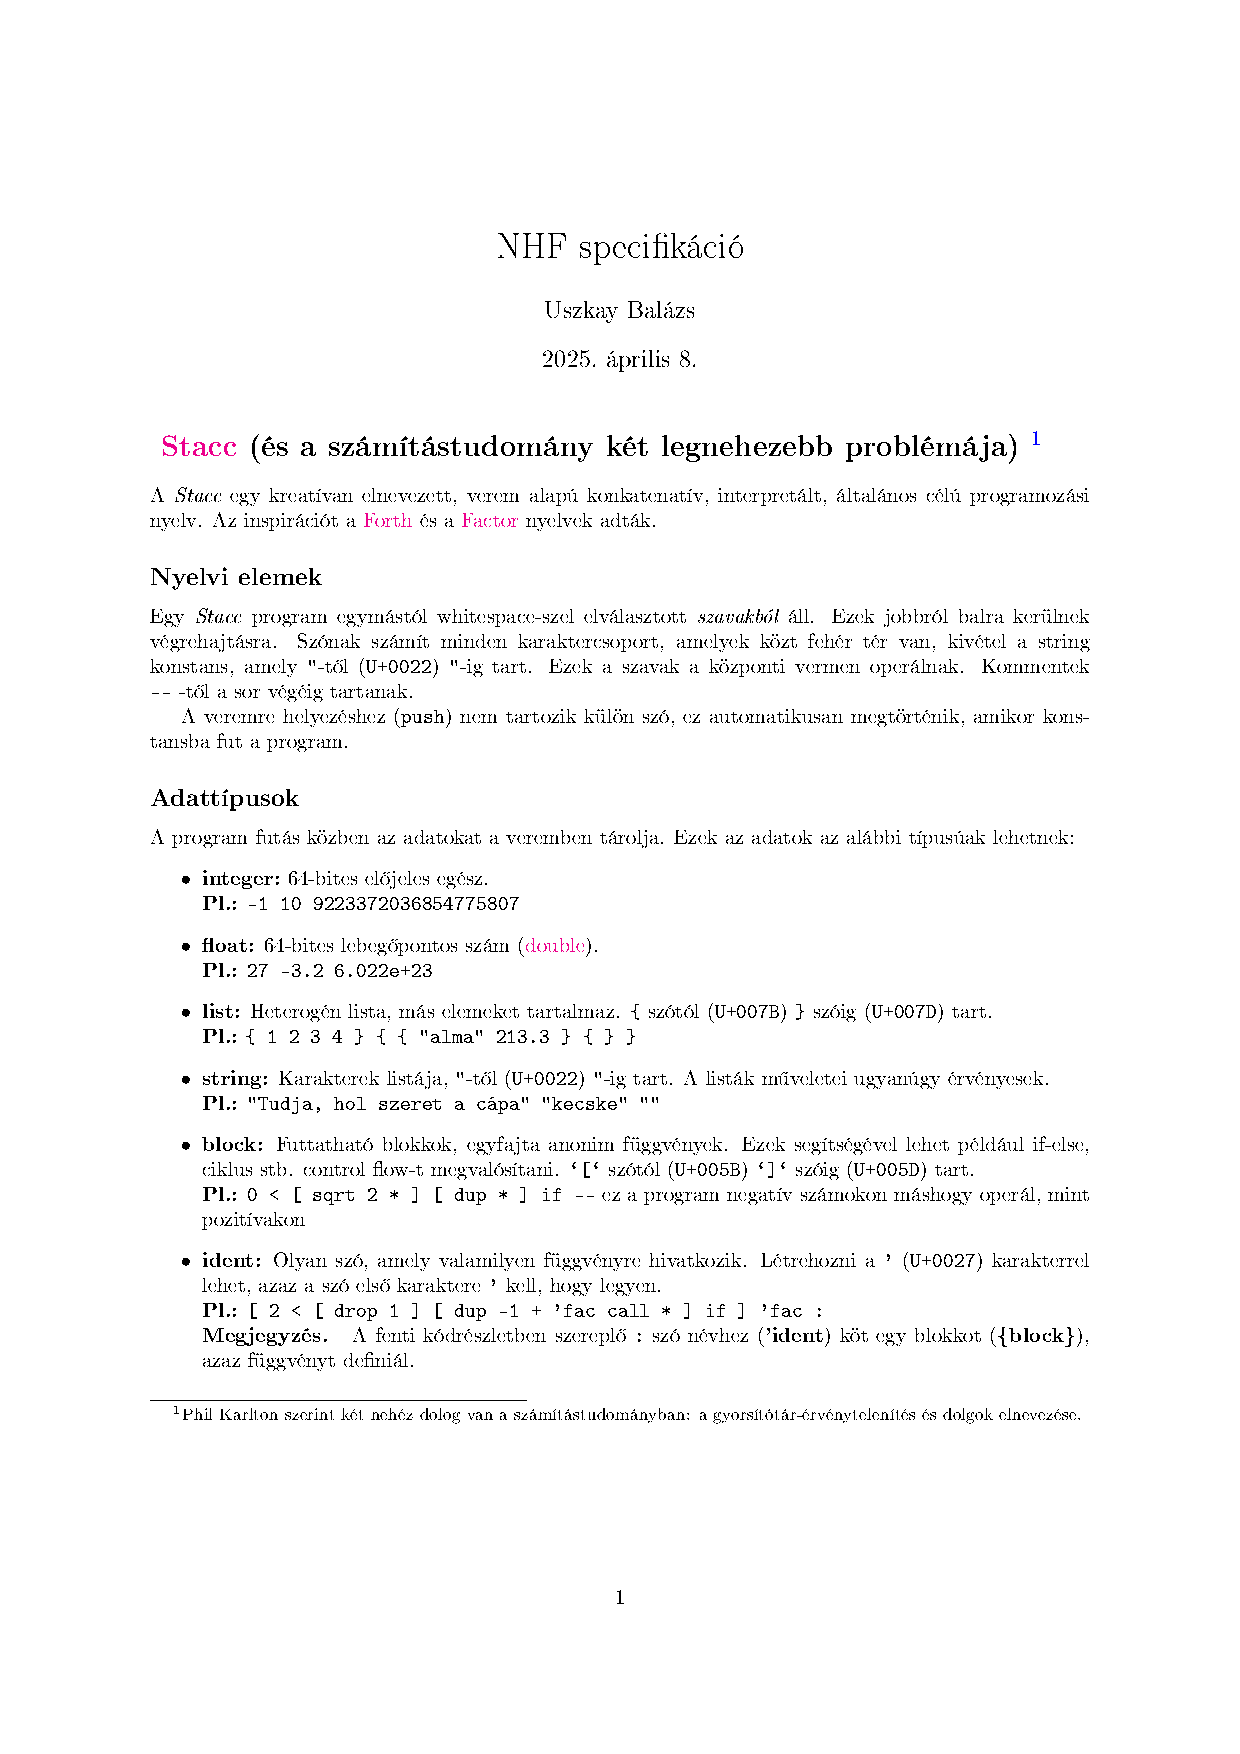
\includegraphics[scale=0.45]{spec.jpg}
\caption{Tervezett osztálydiagram. Ezeken az osztályokon függvények operálnak.}
\end{figure}

\begin{figure}[h]
\caption{Egy program lefuttatásának pszeudokódja.}
\begin{verbatim}
def Futtatas(szoveg: string) -> bool:
    tokenek: Maybe<vector<Token*>> = Tokenize(szoveg).
    if (!tokenek.has_value())
        return true.
    # megjegyzés. ezt a részt vsz. closure-rel oldanám meg.
    objektumok: Maybe<vector<Object>> = Parse(*tokenek).
    if (!tokenek.has_value())
        return true.
    success: bool = Interpret(*objektumok).
    return success.

def Tokenize(szoveg: string) -> Maybe<vector<Token*>>:
    tokenek = empty vector.
    while (szoveg.not_empty()):
        szoveg.skip_ws()
        if (szoveg.next() == '"'):
            olvasd sztringkent, amig ujra nem '"'.
            tokenek.append(uj String(...)).
        olvass be egy szót -> word: string
        ha csak numerikus karakter: 
            tokenek.append(uj Int(word))
        ha lehet valos:
            tokenek.append(uj Float(word))

def Parse(tokenek: vector<Token*>, block: bool=false, list: bool=false) -> Maybe<vector<Object*>>:
    objektumok = empty vector.
    for token of tokenek:
        if block és token == Word(']'):
            return Maybe(objektumok).
        if list és token == Word('}'):
            return Maybe(objektumok).
        if token == Word('['):
            objektumok.append(Parse(tokenek, true, false)).
        if token == Word('{'):
            objektumok.append(Parse(tokenek, false, true))
        objektumok.append(Token típusának megfelelő Object).
    return objektumok.

def Interpret(objektumok: vector<Object*>) -> bool:
    for objektum of objektumok:
        switch objektum:
        | Word('call') > ...
        | Int > ...
        ...
    Ha bárhol hiba van, jelezzük a visszatérési értékkel.

\end{verbatim}
\end{figure}
\end{document}



